\chapter{Results}
    In this chapter we will cover different part of the results. First we will go through the leg pattern motion to see how they move and how accurate they are with previous paper \cite{mo_main_paper}. Then we will focus on the robot displacement and the simulation. 
    \section{Legs patterns}\label{sec:res_legs}
        This is the basic block of results we need in order to build the other modules. We need to be able to encode the 15 sequences that a multistable joint can have as seen on Figure \ref{fig:sequences}. We will go through the sequences here. Each time we will have the same structure, a Figure on the left representing the Final State Machine or the order of motion from the middle and the top block, which can vary from forward and backward movement. On the right we will have a Figure which plot the position of the leg in x-axis and z-axis with respect to the position off the actuator represented by the color of the line.
        \begin{figure}[h]
            \centering
            \begin{subfigure}{.2\textwidth}
            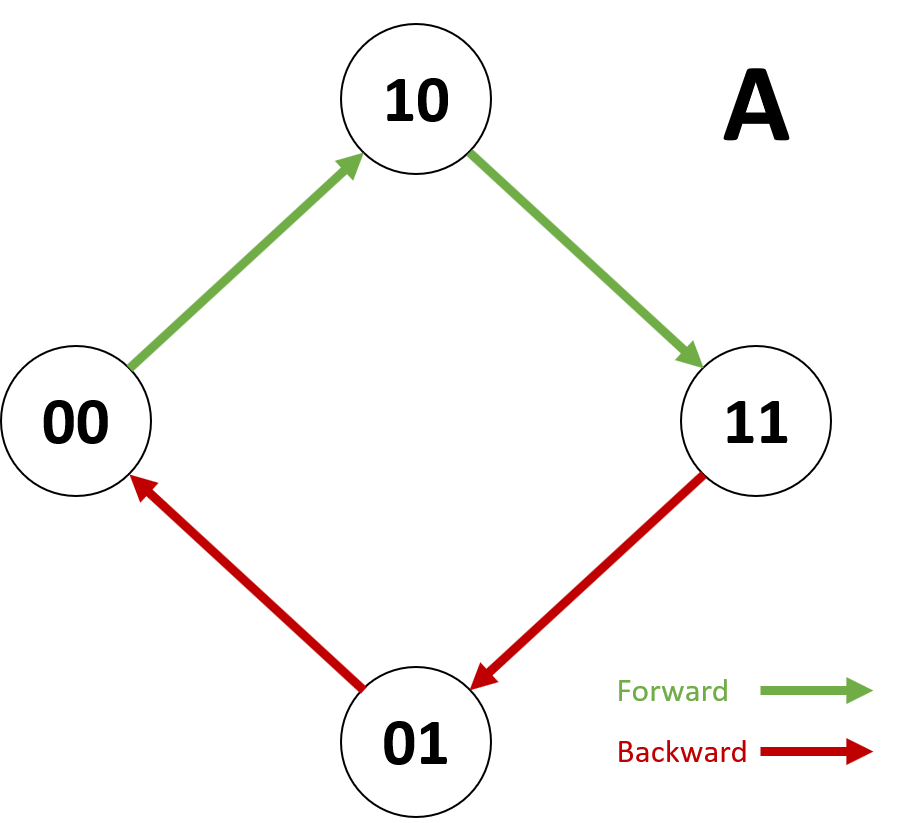
\includegraphics[width=\textwidth]{images/S_A.png}
            \end{subfigure}%
            \begin{subfigure}{.6\textwidth}
            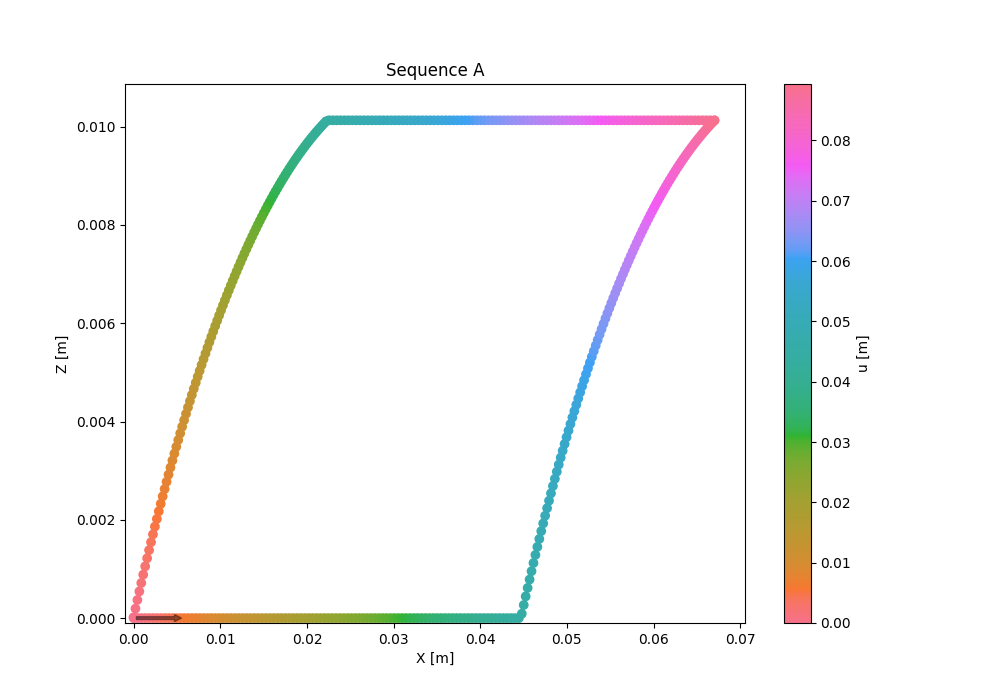
\includegraphics[width=\textwidth]{images/A.png}
            \end{subfigure}
            \caption{Sequence A is one of the simplest sequence where the middle block is moving first in forward and backward motion. This leads to a hysteresis as we can see. The arrow shows the direction of motion, which is counter-clockwise. Sequence B (Figure \ref{fig:appendix_seq_B}) is identical except that it goes clockwise.}
        \end{figure}
        
        
        \begin{figure}[h]
            \centering
            \begin{subfigure}{.2\textwidth}
            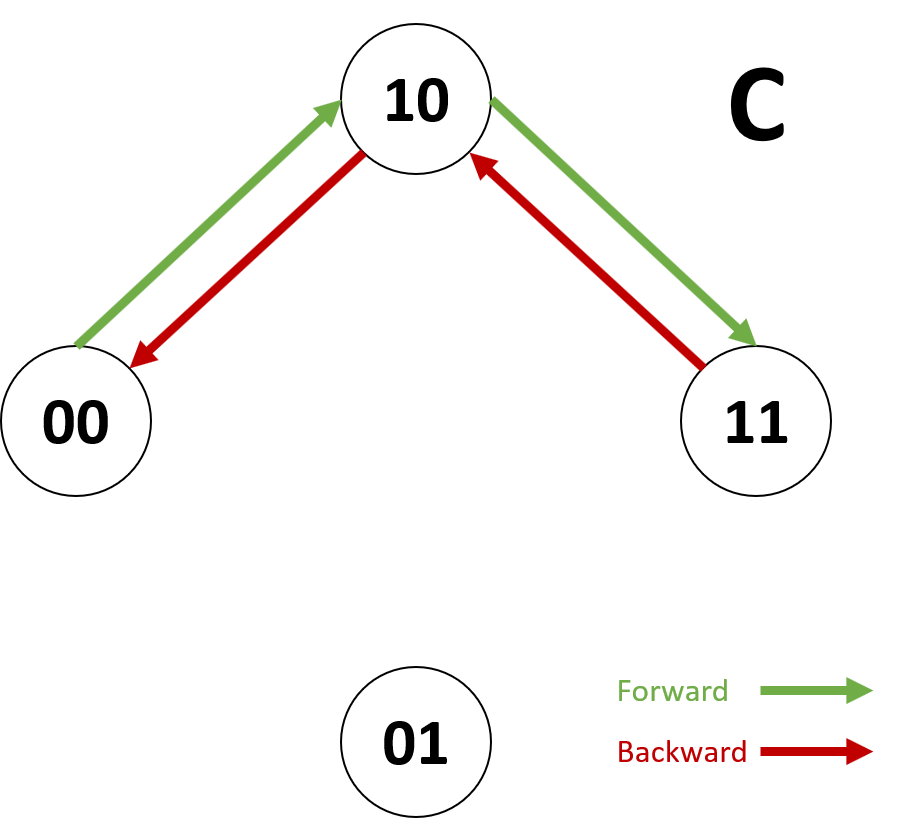
\includegraphics[width=\textwidth]{images/S_C.png}
            \end{subfigure}%
            \begin{subfigure}{.6\textwidth}
            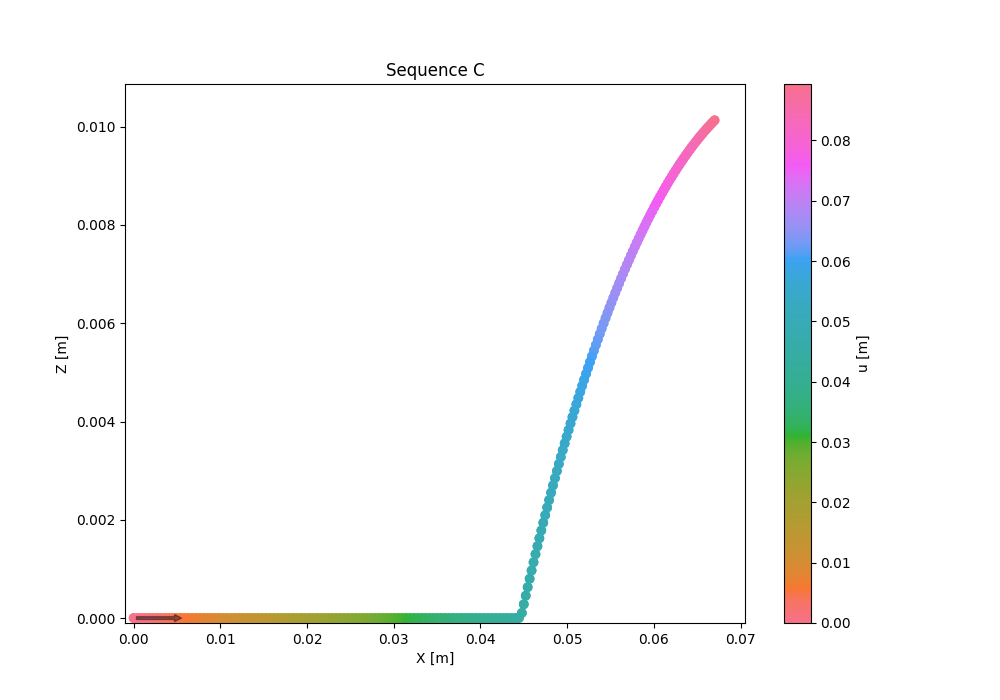
\includegraphics[width=\textwidth]{images/C.png}
            \end{subfigure}
            \caption{Sequence C is a symmetrical sequence where the forward and backward motion are following the same path. In this sequence we have first the middle block moving during the forward motion where the top block is moving first during the backward motion. Sequence D (Figure \ref{fig:appendix_seq_D}) is very similar except it is reversed.}
        \end{figure}
        
        \begin{figure}[h]
            \centering
            \begin{subfigure}{.2\textwidth}
            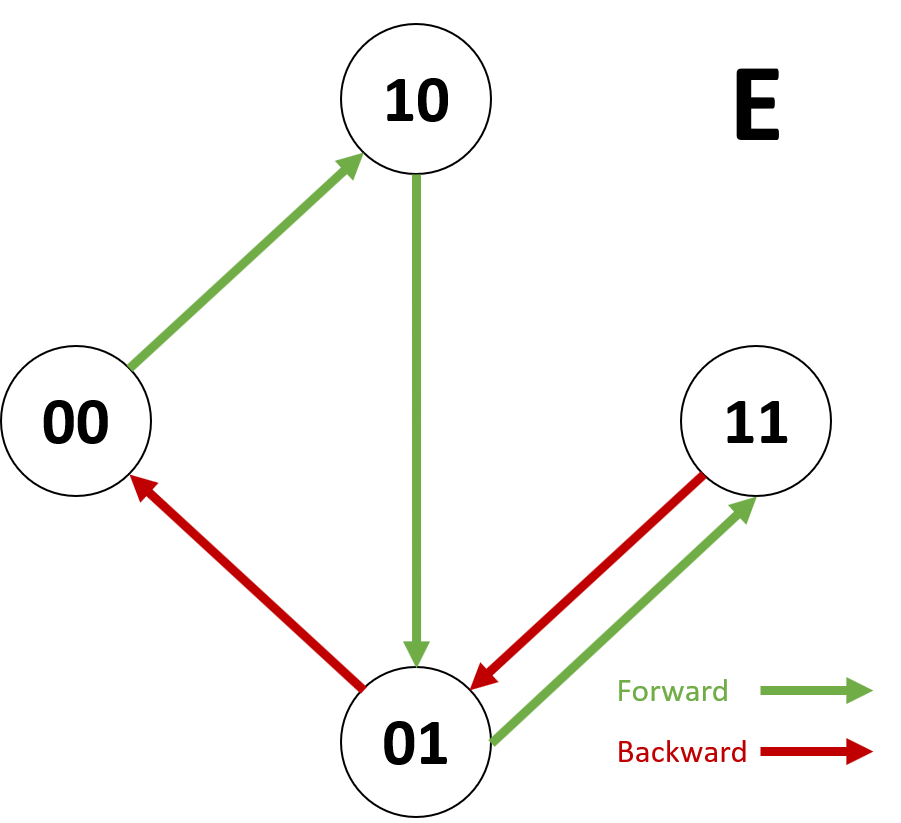
\includegraphics[width=\textwidth]{images/S_E.png}
            \end{subfigure}%
            \begin{subfigure}{.6\textwidth}
            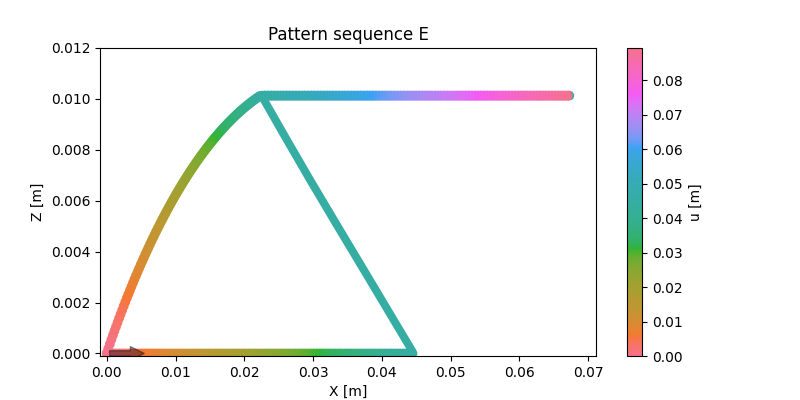
\includegraphics[width=\textwidth]{images/E.png}
            \end{subfigure}
            \caption{Sequence E is our first sequence with a avalanche mechanism where two blocks swap positions. This happens in the middle of the forward motion. We can see here that after moving horizontally, the legs is \textit{snapping} to go to another position without having motion for the actuator, producing this triangle shape. Sequence F (Figure \ref{fig:appendix_seq_F} is performing similarly but \textit{reversed}.}
        \end{figure}
        
        \begin{figure}[h]
            \centering
            \begin{subfigure}{.2\textwidth}
            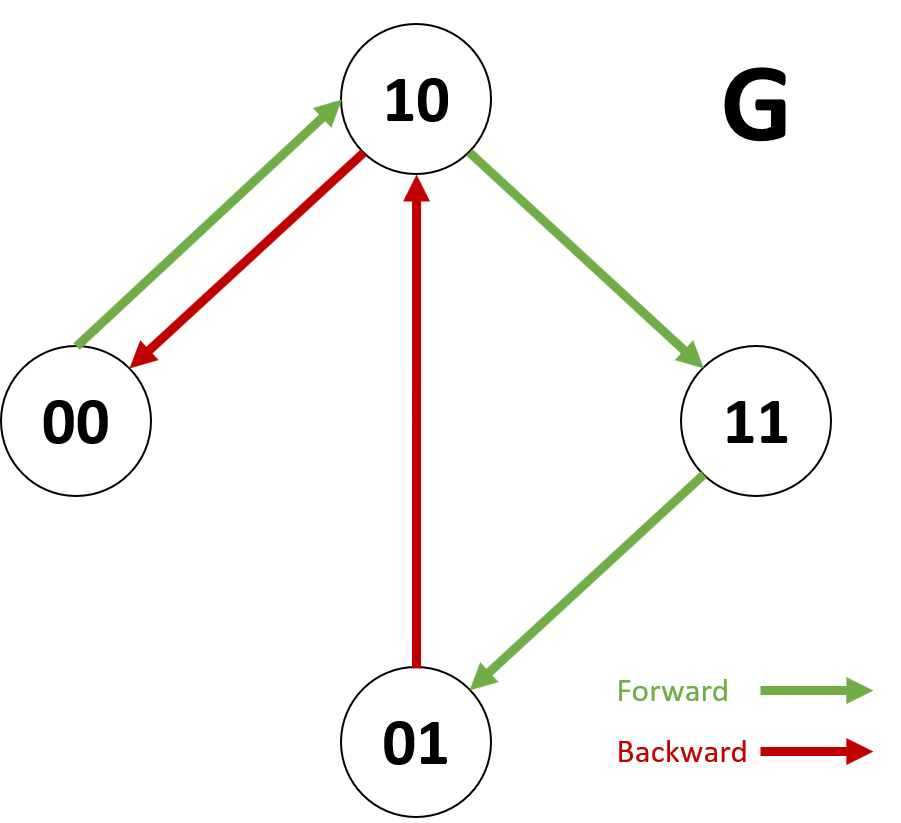
\includegraphics[width=\textwidth]{images/S_G.png}
            \end{subfigure}%
            \begin{subfigure}{.6\textwidth}
            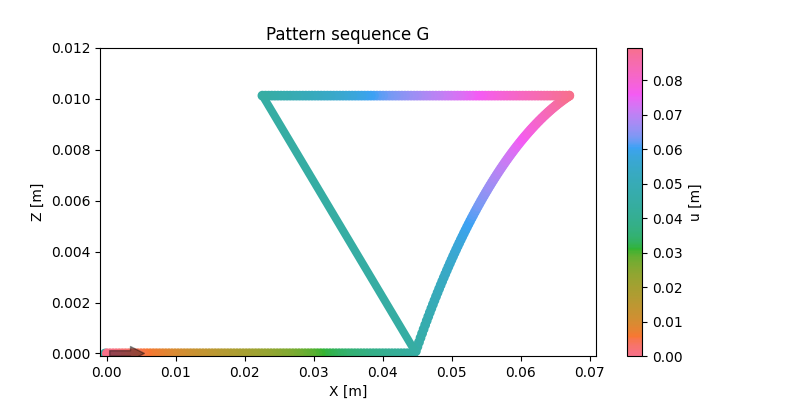
\includegraphics[width=\textwidth]{images/G.png}
            \end{subfigure}
            \caption{Sequence G is similar to sequence E and sequence F as there is also an avalanche effect that swap two blocks positions. But this time this swap motion happens during backward actuation instead of forward actuation. Sequence H (Figure \ref{fig:appendix_seq_H} is performing similarly but \textit{reversed}.}
        \end{figure}

        \begin{figure}[h]
            \centering
            \begin{subfigure}{.2\textwidth}
            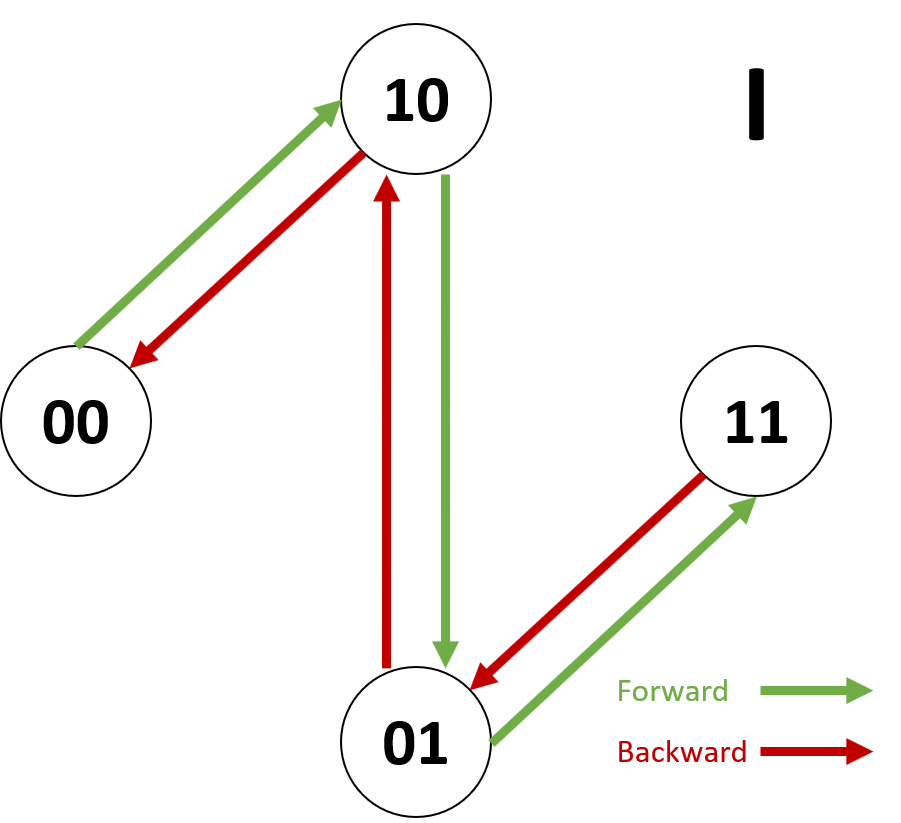
\includegraphics[width=\textwidth]{images/S_I.png}
            \end{subfigure}%
            \begin{subfigure}{.6\textwidth}
            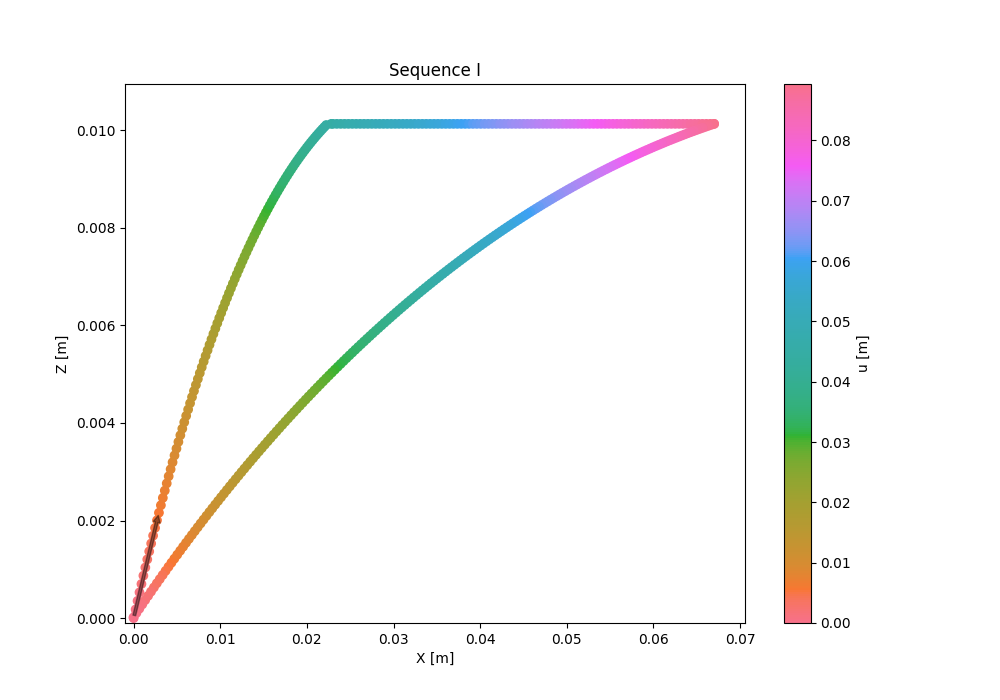
\includegraphics[width=\textwidth]{images/I.png}
            \end{subfigure}
            \caption{Sequence I is our only sequence with two avalanches mechanisms. This time we can see that the two blocks swap positions during forward and backward motions.}
        \end{figure} 
        
    \section{Robot behavior visualization}
        Let's show what information are shown in the video of the simulation. We have an example of the kind of video you can expect as a result in Figure \ref{fig:drawing}. The simulation represent the robot in a schematic way, with a main frame represented by yellow blocks. On each corner we have a multistable joint as for the real robot. Actuators are not directly represented but we can identify two type of top blocks, green ones and magenta ones. Top blocks with the same color are linked together to the same actuator. Linking the blocks together we have springs and arms, respectively in gray and red. 
        
        \begin{figure}[h]
            \centering
            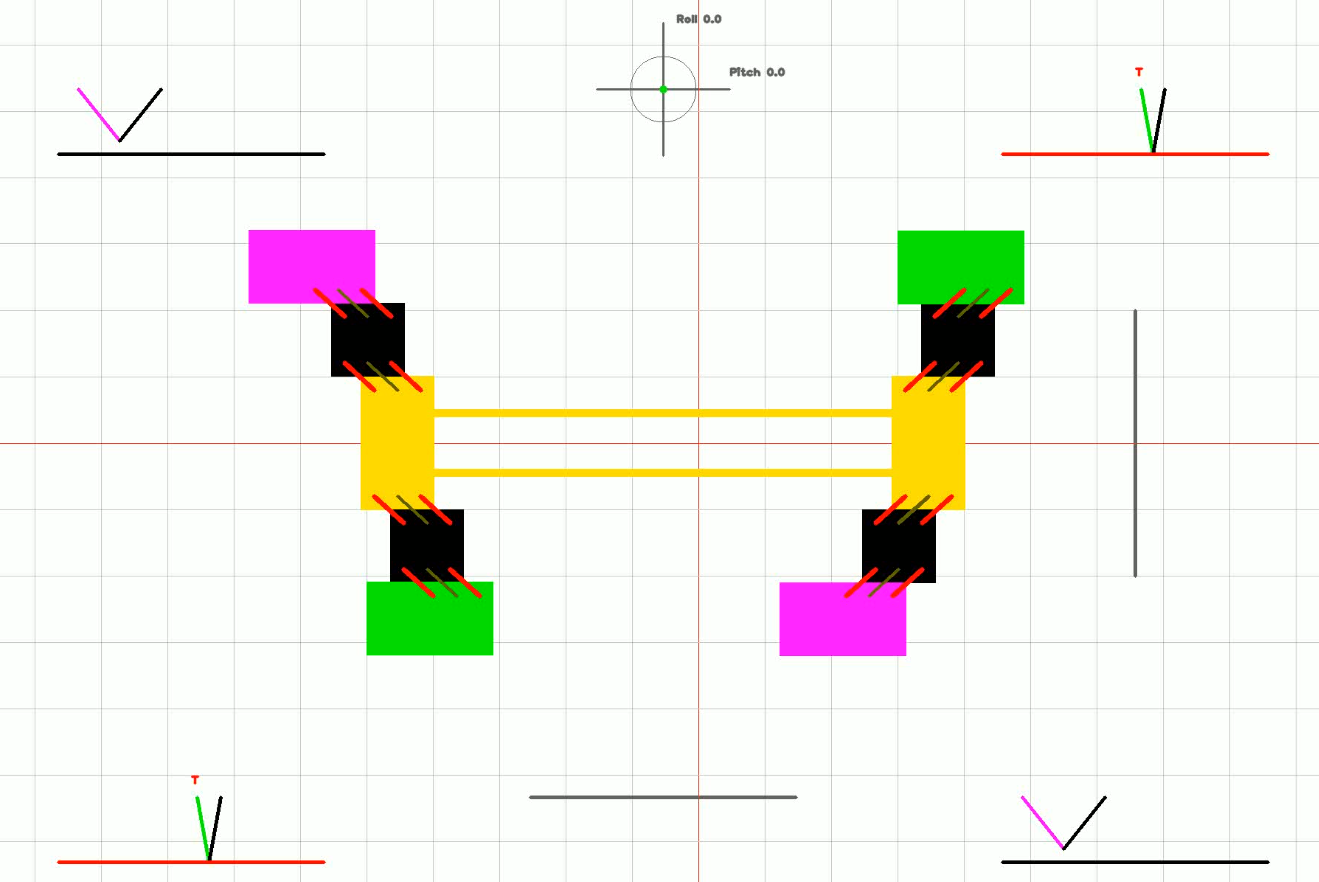
\includegraphics[width=0.8\textwidth]{images/drawing.png}
            \caption{We can see an example of the type of drawing the simulation produces. It is mainly a top view of the robot, with the frame in yellow, and the four multistable joints. The actuators are not represented directly but we can determine which top blocks are linked together by color. Green blocks are linked together, and magenta blocks are linked together. On the four corners we can see a side view of the respective leg, with an horizontal line that represent the ground relative to the foot. This line is in black when the foot is not touching the floor, and in red when it is. on the top of the image, we can see a representation of the pitch and roll angle of the main frame relative to the ground. this is also duplicated with the vertical line on the right and the horizontal line on the bottom of the picture, which represent a side view of the robot. The background of the image consists of a grid with a reference of the origin with a red cross. It is used to visualize how the robot is moving relative to the floor.}
            \label{fig:drawing}
        \end{figure}
        
        The view of the robot is a top view as it allows us to understand how the sequences are happening. We have four smaller views on the four corner of the image. Those view represent a side view of each multistable joint. If we take the the example of the bottom left leg, we have a horizontal line which is a virtual representation of the ground position relative to the leg. We also have a green and black lines, the green line represent the arm that link the green block to the leg endpoint. The block line represent the arm that link the black block to the leg endpoint. The letter T and the red line are present when the leg is in contact with the ground. We can see in our case that two (green) legs are touching the ground while two others (magenta) are not.
        
        We can also see on top of the image a cross with a green dot. This is one way to represent the attitude of the robot, in particular the pitch and roll rotation. Pitch rotation will be positive when the front of the robot (on the right) is lower than the rear of the robot (on the left). Similarly for the roll axis. We also have a second representation of the inclination of the robot with a vertical line on the right of the image that will be tilted with the roll rotation and the horizontal line on the bottom of the image that represent the pitch rotation.
        
        On the background of the image we have a grid in gray to see how the robot is evolving compare to the ground. And to have a reference we have a red cross in the background that represent the origin of our virtual world. 
        
    \section{Robot trajectory}\label{sec:res_position}
        The simulation also output a graph with the position of the robot relative to the cycle(s). As we can see on Figure \ref{fig:robot_position}, we have the x-axis and y-axis displacement of the robot on the first subplot and the orientation change in the second subplot, this correspond to the heading of the robot. The horizontal axis is without unit but instead we grid it using cycle.
        \begin{figure}[h]
            \centering
            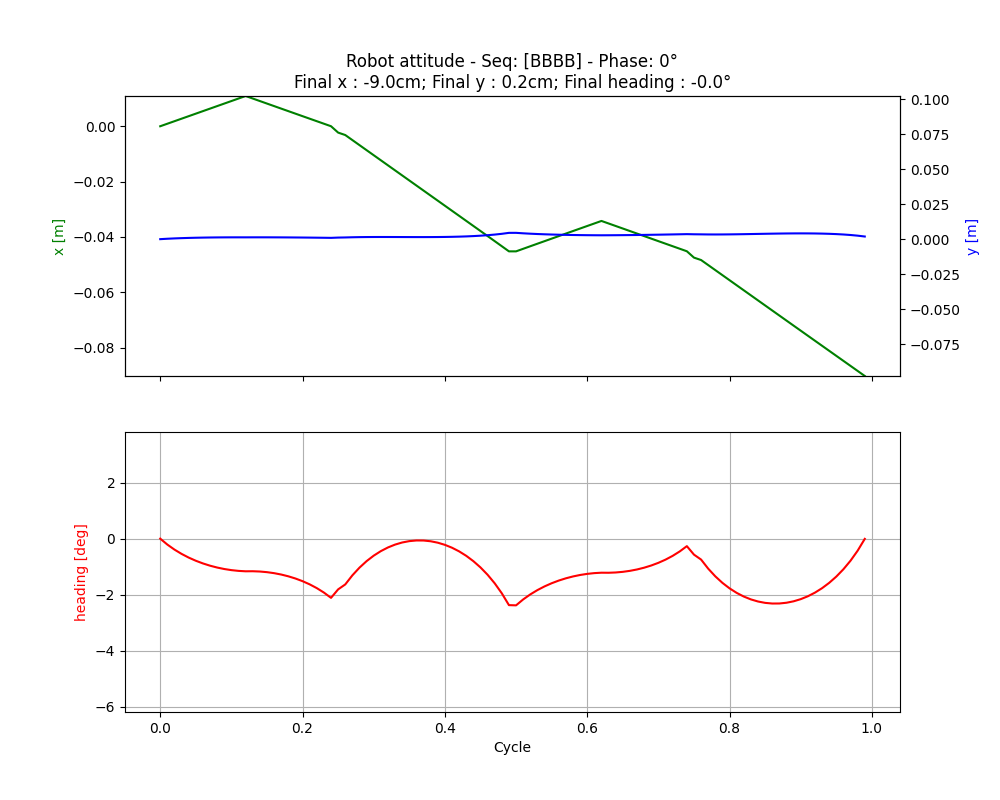
\includegraphics[width=0.7\textwidth]{images/robot_position.png}
            \caption{An example of output produced by the simulation that tracks the position and the orientation of the robot during the cycles. We can see the x-axis displacement (horizontal in videos) and the y-axis displacement (vertical in videos). Also we see the orientation change of the robot, which correspond to the heading. This plot has been generated using sequence \textit{BBBB} with a phase difference of $0$°}
            \label{fig:robot_position}
        \end{figure}
    
    \section{Displacement mapping}\label{sec:res_mapping}
        Now that we have a simulation for different parameters, we can create a map of motion for all the different sequences. Each leg can be programmed to act with one of the 10 sequences and we can have a phase difference of 0° or 180°. This gives $20'000$ combinations. To create a correct symmetry we will also switch the starting position of the actuators, which gives a total of $40'000$ combinations. Each combinations will produce a x-axis and a y-axis displacement for the robot and a change in orientation that we can represent in a table. The table produced contain then $40'000$ rows and $6$ columns containing the sequence, actuation phase and starting point as input and the displacement of the robot (x, y, heading).
        
        \begin{figure}[h]
            \centering
            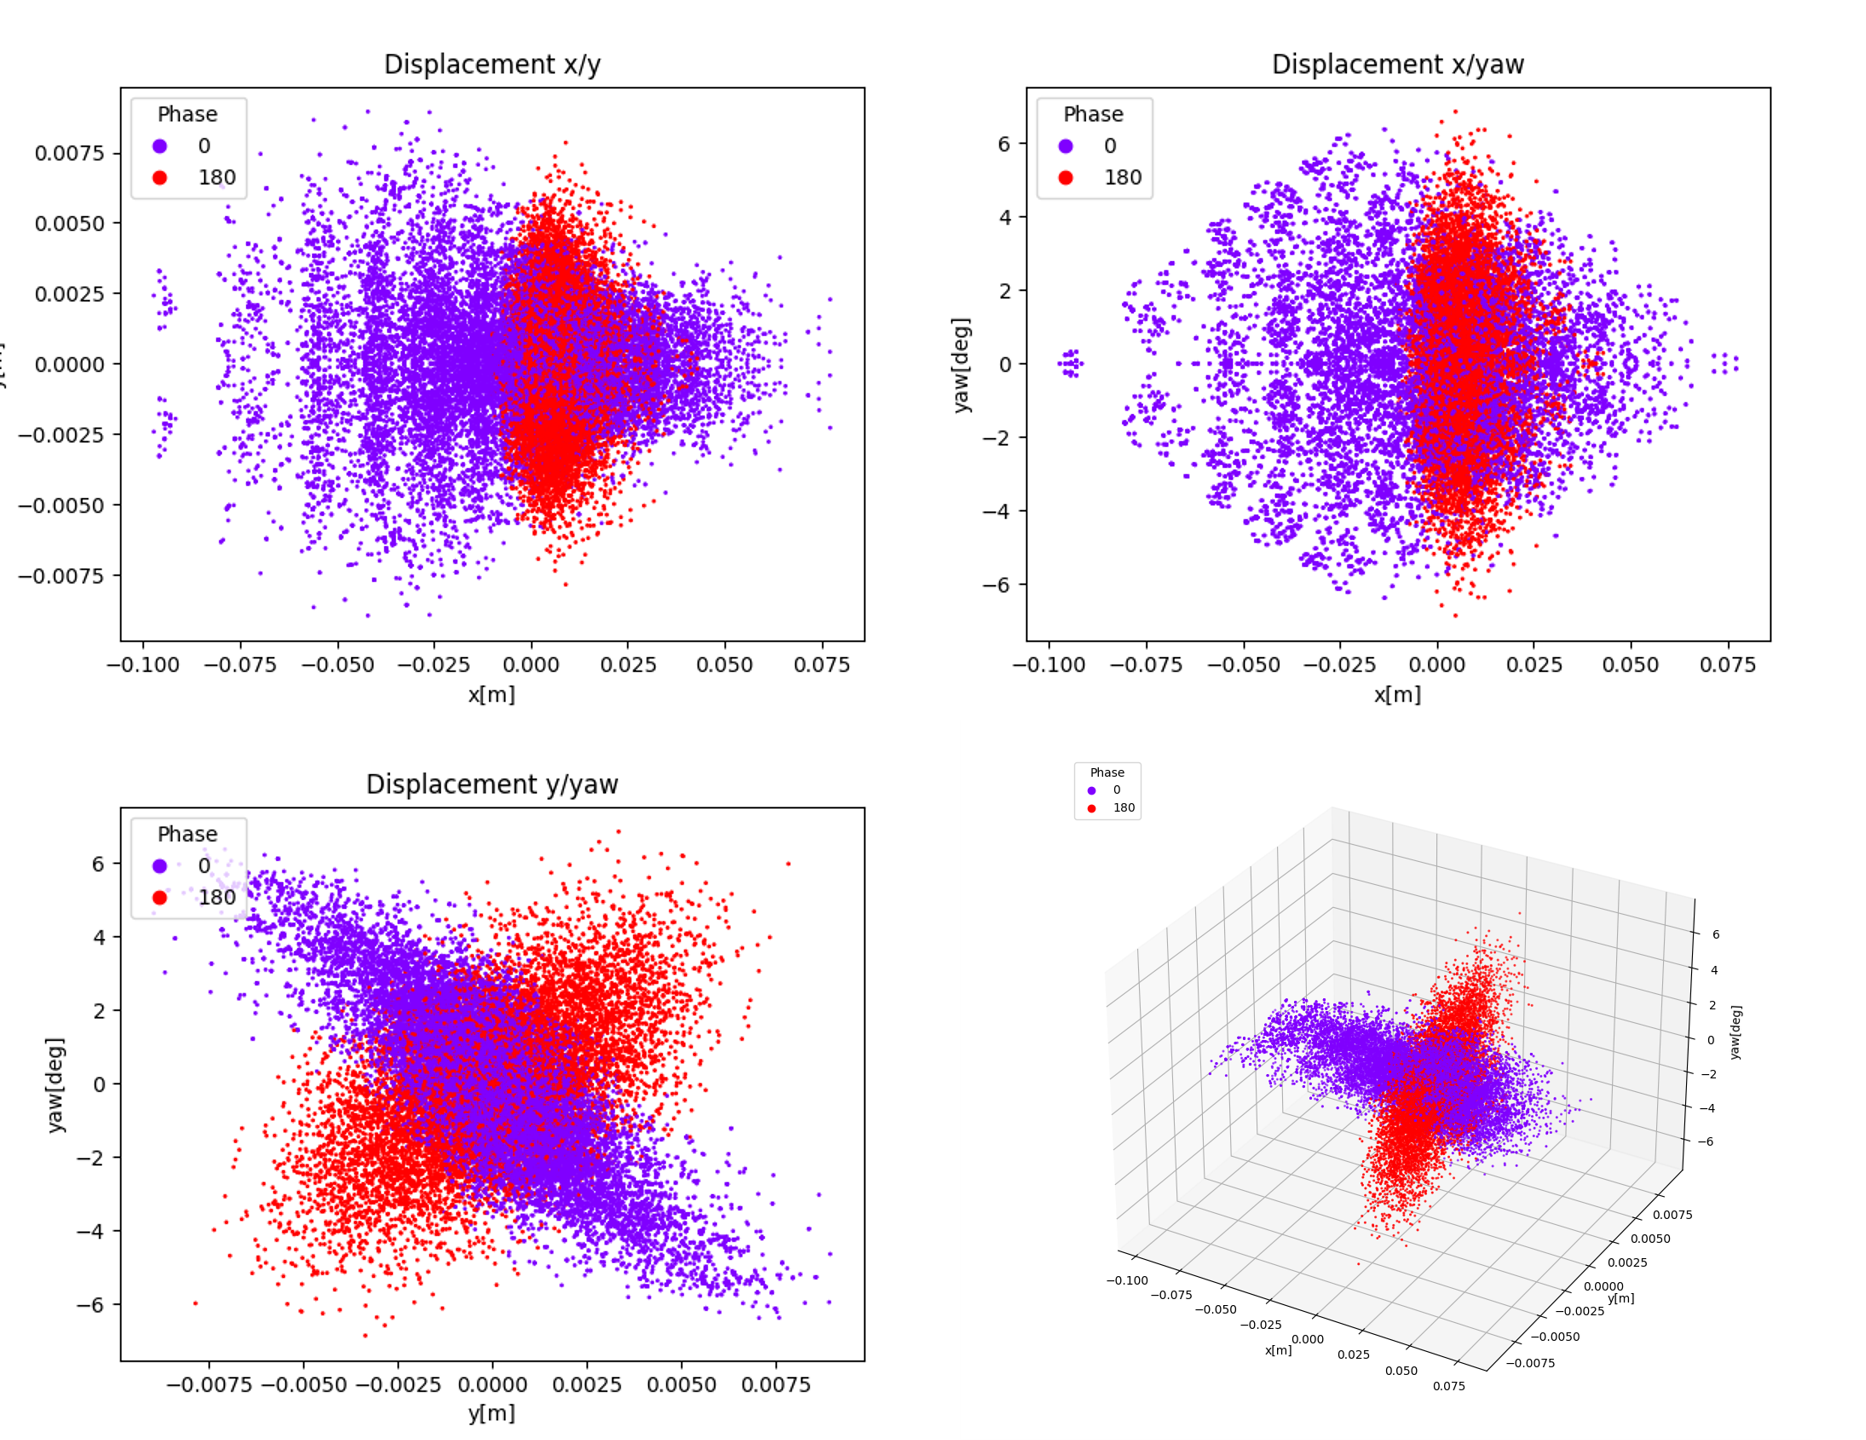
\includegraphics[width=0.66\textwidth]{images/displacement_spread.png}
            \caption{Multiple view of the possible motion of the robot. The robot can move along x-axis and y-axis, but also change its orientation. Bottom right plot shows the 3D view of the $40'000$ possible sequences. Other plots are a projection of those point on only 2 axis. Red dots are sequences with a 180° phase difference while purple dots are sequences with no phase difference.}
            \label{fig:displacement_spread}
        \end{figure}
        
        We can see on Figure \ref{fig:displacement_spread} the spread of displacement and orientation for the $40'000$ different sequences (A-J) with two different color depending on the phase difference applied. Red dots represent a phase difference of 180°, corresponding to the actuators extending and retracting in opposition.
        
    \section{Deep Q Learning Results}\label{sec:res_qlearning}
        The Deep Q Learning controller is able to learn how to select sequences to drive the robot to a specific place. Figure \ref{fig:dqn_results} shows an example of learning process for a robot restricted to use sequence A or B for each legs. On the Figure a plateau is created after 40 iterations where the number of steps stabilize around 200 and the number of sequence change for the scenario stabilize around 35. The results also include multiple videos where the controller is shown in action and complete the tasks.
        \begin{figure}[h]
            \centering
            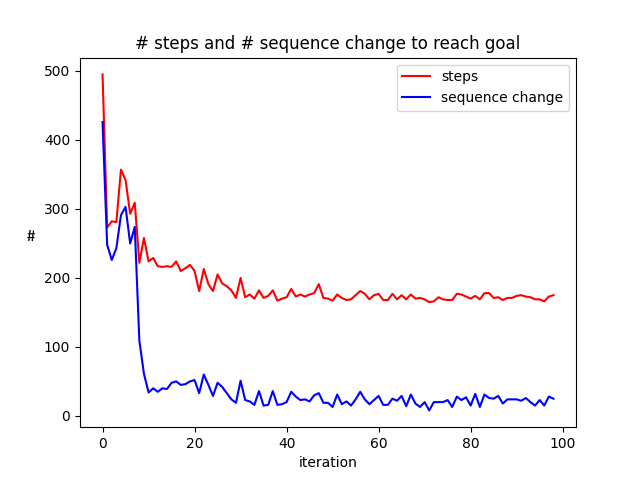
\includegraphics[width=0.7\textwidth]{images/AB-0-FALSE.png}
            \caption{Learning process of a Deep Q Learning Controller. Two lines represent the progression, red line is the number of steps done for each iteration to reach the goal. The blue line represent the number of sequence change that occur during the iteration. Each iteration consist of the same scenario but with different starting orientation (which is the end orientation of the previous scenario). The robot was restricted to use only sequences A and B.}
            \label{fig:dqn_results}
        \end{figure}
        
        Figure \ref{fig:all_sequences} shows the learning progress of a similar Deep Q Learning (two layer of hidden layers instead of one), but instead of restricting to some sequences, the neural net is given all the possible sequences. Again the red line represent the number of steps required for the iteration and the blue line represent the number of switches.
        
        \begin{figure}
            \centering
            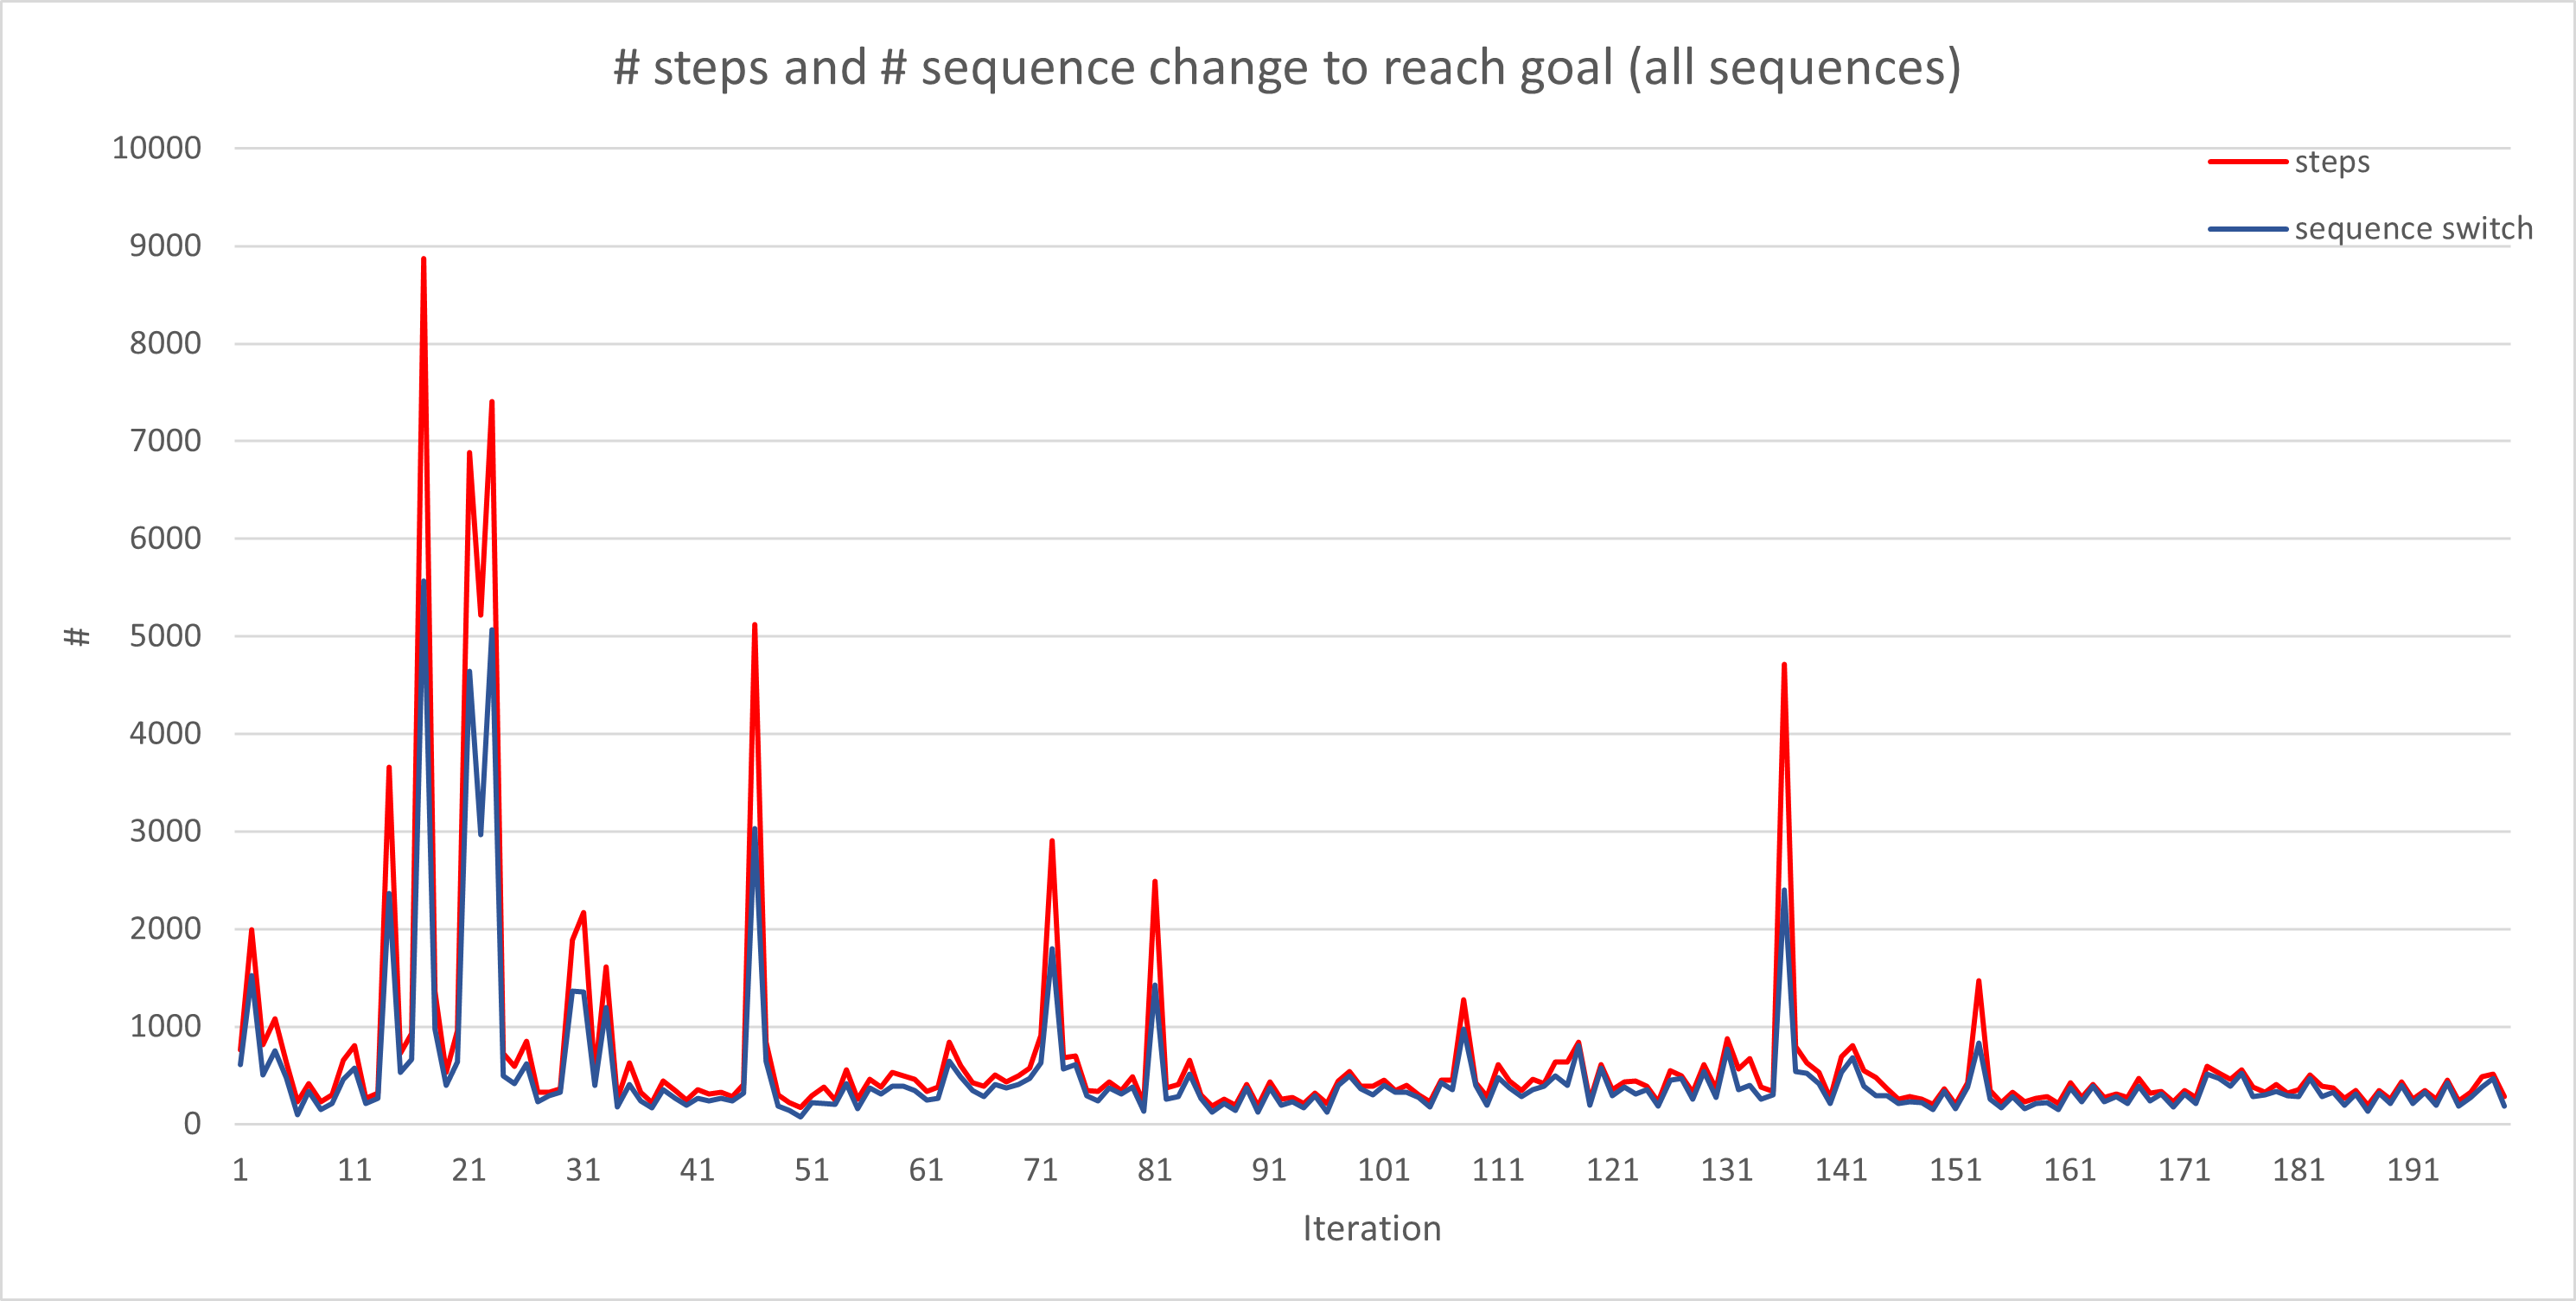
\includegraphics[width=0.9\textwidth]{images/ALL_SEQ_QLEARN.png}
            \caption{Example of Deep Q Learning process with all the sequences enabled. Red line represent the number of steps to reach to the iteration target. Blue line represent the number of sequence changes done during the iteration.}
            \label{fig:all_sequences}
        \end{figure}
        